\subsection{第 4 课 | 栈、队列、优先队列、双端队列}

\subsubsection{脑图}

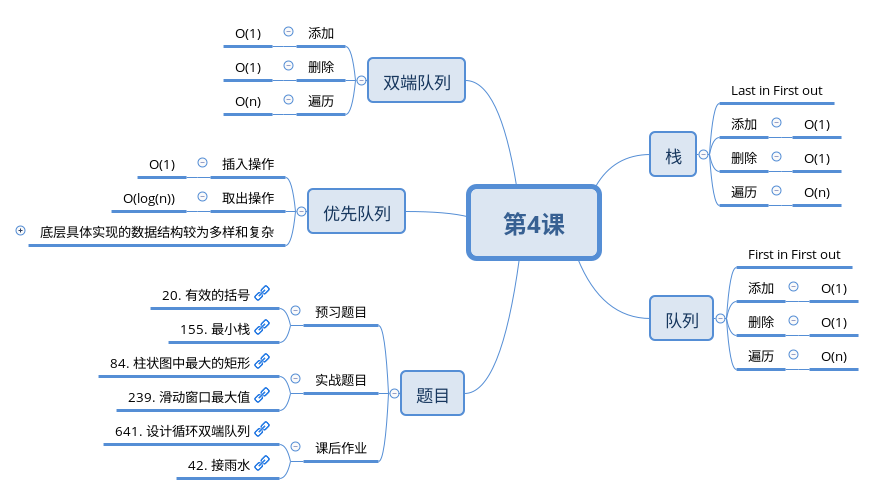
\includegraphics[width=170mm,height=80mm]{images/camp/第4课.png}

\subsubsection{题目}

\paragraph{预习题目}

\begin{itemize}
  \item \hyperref[leetcode:20]{20. 有效的括号}
  \item \hyperref[leetcode:155]{155. 最小栈}
\end{itemize}

\paragraph{实战题目}

\begin{itemize}
  \item \hyperref[leetcode:84]{84. 柱状图中最大的矩形}
  \item \hyperref[leetcode:239]{239. 滑动窗口最大值}
\end{itemize}

\paragraph{课后作业}

\begin{itemize}
  \item \hyperref[leetcode:641]{641. 设计循环双端队列}
  \item \hyperref[leetcode:42]{42. 接雨水}
\end{itemize}
